% Authorship: Claude-drafted, author-revised
\section{The Static Model Is Sound}

Given faithful weights, stipulated here, not yet grounded in any
practice, does the aggregation Berman describes do what the theory needs?
It does, and the sharpest evidence arrives before any weight is tuned. Put a hard conflict to a Hartian validation rule, a recognition apparatus that
asks of each authority only whether it is valid and which way it points, and
the rule certifies both sides at once: each authority is valid, each points a
way, and both outcomes come back as legally required. The weighted sum
cannot do this. Because summing weighted forces yields one net force with one sign, it
returns at most one verdict. On directly opposed cases the validation rule contradicts itself every time
and the weighted sum never does. Though the two halves are not established in
the same way, neither is a lucky run. As an entailment of the
aggregation form, the sum's coherence holds on any case whatever, while the
rule's failure follows from the structure of any case in which principles
apply strongly on both sides. Each is stated below with the scope it is
proved under.

Beyond that, the stipulated engine of Part III, run on weights set by hand
rather than conferred by practice, is the static model of this Part's title,
and it has three further virtues the theory asks of it: it tolerates rough weights, it weighs the magnitude of competing principles,
and it leaves less law unsettled than a tiered Hartian hierarchy, which is a
second and different rival taken up below. Of the four, though, the contradiction is the one to keep in view: where
the validation rule contradicts itself, the weighted sum still answers.

Throughout, the organizing frame is the four requirements of Part~III, that
the weights be well-defined, that they tolerate rough specification, that
the model weigh magnitude rather than rank by fixed priority, and that it
deliver more law than Hart, together with the claims of Berman's they track.
Here the first of the four requirements is met by stipulation, since weights
supplied by hand are well-defined by construction, and it becomes a live test
only in Part~V, where practice has to supply them. This Part puts the other
three to work.

Rough weights and conflict come first, then the Hart advantage, then
magnitude-weighing, and last the load-bearing claims restated as theorems.
Deferred are two questions the static analysis raises but does not settle.
How much of the law comes out determinate turns on the threshold, and that
belongs to Part~VIII. How far the weighted sum departs from ordinal
alternatives is for Part~VII.

One convention governs every number below. Here the cases are synthetic and their activations drawn independently,
which is the conservative choice. In reality cases are correlated, and
correlation, as the next Section measures, more than doubles the model's
tolerance for weight error. Read the determinacy rates that follow as floors: they are what the weighted
sum achieves when the data are least favorable to it, and at the
correlation this Article treats as realistic it does better. Since the
conflict batteries are built by construction rather than drawn, the conflict
numbers are not floors in that sense, and no correlated counterpart to them
was run. The convention does not
extend to the margin over Hart, and the exception is not small. Under
category-correlated activations, where principles of the same category tend to
point the same way, that margin reverses, for reasons the Hart comparison
below takes up.

\subsection{Rough Weights Suffice, and Conflict Does Not Defeat Them}

However the theory is read, it cannot require exact weights, and Perry's
objection is that practice could never supply them.\footnote{See Perry, \textit{supra} note 9, at 794.} Berman's reply is that rough weights suffice,\footnote{Berman,
\textit{Practices}, \textit{supra} note 7, at 328--30.} and the model appears to bear him out. Sweeping a grid of forty-five configurations (three weight
distributions, three principle counts, five determinacy thresholds), the
weighted sum tolerates a mean critical uncertainty of $\sigma^{*} \approx
0.090$, ranging from $0.071$ to $0.134$.\footnote{Recall from Part~III that
$\sigma^{*}$ is the level of Gaussian weight perturbation at which one case
in five flips its signed verdict; each configuration uses thirty seeds,
reported with 95\% bootstrap confidence intervals.} Before the verdicts begin
to move, each weight can apparently be wrong by about this much. If the true weight of human
dignity is $0.80$, the model returns the same verdicts so long as practice
places it anywhere from roughly $0.71$ to $0.89$, the distance between
``quite important'' and ``very important.'' That is the tolerance Perry
doubted aggregation could have.

That tolerance is also where Part~III's noise-tolerance floor comes from. Set just below
the lowest of the grid's forty-five configuration means, the $\sigma^{*} \geq
0.07$ requirement asks an emergent mechanism to be about as robust as the
stipulated engine is on average at its least robust setting. It does not ask
it to beat the engine's worst run. On larger samples that run falls below the
floor more often than not.

These figures assume independent activations, the conservative baseline
announced at the outset, and correlated activations raise them. In real cases principles point together within a category, textual with
textual, moral with moral. Category-correlated activations more than double the tolerance for weight
error, raising $\sigma^{*}$ from $0.069$ to $0.156$ in a paired run held at
nine principles, moderate weights, and a determinacy threshold of
$\tau = 0.2$.\footnote{Category correlation raises $\sigma^{*}$ on every one of the thirty seeds. The
pair comes from a separate run rather than from the forty-five-configuration
grid, on eight hundred cases rather than that grid's three hundred and with
sixty-four noise redraws rather than forty, and its independent baseline of
$0.069$ sits a shade below that grid's $0.071$ for the same configuration. The
gap is within the grid cell's own confidence interval, which runs from $0.068$
to $0.073$. Within the pair the sample, the redraw count, the noise draws, and
the weights are all held fixed, so what the comparison isolates is the
difference between the two activation structures, not a new floor. Under
full correlation $\sigma^{*}$ runs past the top of the tested grid, so it
can be reported only as a lower bound.} Correlation lifts the
tolerance and the determinacy rate, not every quantity in this Part; the
margin over Hart moves the other way, as the next Section reports.

Across the grid, the little variation in $\sigma^{*}$ comes almost
entirely from the threshold, not the weight distribution: roughly $84\%$ of
the spread traces to the choice of $\tau$, against about $14\%$ for principle
count and $2\%$ for the weight distribution.\footnote{The spread in
$\sigma^{*}$ attributable to threshold choice is $0.049$, to principle count
$0.008$, and to weight distribution $0.001$.} That the weight distribution
barely moves the model's tolerance is the rough-weights claim from another
angle. Determinacy trades against the threshold, analyzed in
Part~VIII.

When principles agree, rough weights are easy to tolerate; the test is
conflict. I sort cases into four types: aligned (all principles favor one side),
opposed (half strongly favor, half strongly oppose), balanced (an even
split at moderate strength), and random. At a demanding threshold ($\tau =
0.2$) I then measure determinacy. Aligned cases are decided every time,
random cases $86.4\%$ of the time, and the hard cases, opposed and balanced,
$51.9\%$ and $55.9\%$.\footnote{Determinacy rates at $\tau = 0.2$ across
thirty seeds; aligned cases decide at a rate of $1.00$. The contradiction
comparison is the first of the five results collected in Section~IV.D.} Those last two are the numbers that
matter, and the rival makes them matter, not the
threshold. On these same opposed cases the validation rule of the opening decides
none of them coherently: it certifies both sides of every one. Half of the hardest conflicts decided, against a rival that contradicts
itself on every one, is arguably a stress test passed rather than merely
survived.

At the baseline Berman
himself endorses, deciding by the bare sign of net force ($\tau = 0$), the
weighted sum resolves nearly every conflicting case but those in genuine
equipoise.\footnote{Berman is explicit that an aggregative system need not
impose any confidence threshold and may decide on the bare balance. See
Berman, \textit{Practices}, \textit{supra} note 7, at 331; \textit{supra}
Part~II.A. The threshold is a confidence gate examined in Part~VIII, not a
quantity the theory fixes.} Where the sum does not decide, it returns honest
indeterminacy rather than contradiction: the cases in or near equipoise,
reported as unresolved rather than resolved both ways at once. Conflicting
principles, in this sense, coexist.

Figure~\ref{fig:f1-static} draws the contrast directly. On the left, the validation rule contradicts itself across the opposed
battery while the weighted sum returns a single verdict throughout. The sum's determinacy there is about $52\%$, the opposed cell reported above,
remeasured on a larger draw from the same generator. On the right, the
model works three real disputes.

\begin{figure}[t]
\centering
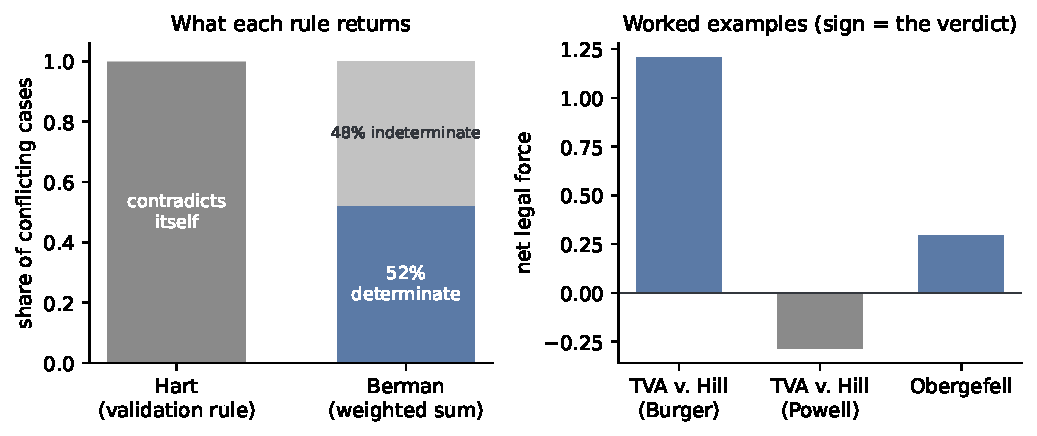
\includegraphics[width=\textwidth]{F1_static_saw}
\caption{The static weighted sum. \textit{Left}: on six thousand opposed
cases, the hardest conflict type, a Hartian validation rule contradicts
itself on $100\%$ of them, certifying both outcomes at once; the weighted
sum never contradicts itself, deciding about $52\%$ at $\tau = 0.2$ and
reporting the rest as unresolved. Thirty-seed means. The sum's coherence
holds as an entailment; the rule's $100\%$ is the rate on cases built to be
directly opposed, and on unstructured draws it is $45.4\%$; the determinacy
rate is measured throughout. See Section~IV.D. \textit{Right}: net legal force
on three worked examples, the sign giving the verdict. \textit{TVA v.\
Hill} returns $+1.205$ under Burger and $-0.285$ under Powell, opposite
determinate verdicts on one statute, and \textit{Obergefell} returns
$+0.295$.}
\label{fig:f1-static}
\end{figure}

Run through the stipulated weights of Part~II, these three disputes would seem to show the model tracking the balance rather than
manufacturing it. \textit{TVA v.\ Hill}
under Chief Justice Burger's activations produces a net force of $+1.205$, a determinate verdict. Under Justice Powell's activations the same case produces $-0.285$,
determinate the other way. That one case
lands on opposite sides of the line under two sets of activations is the opposite of
a curated demonstration: weights chosen to flatter the model would not
reproduce the split the bench actually reached. \textit{Obergefell} produces
$+0.295$, determinate.\footnote{The full \textit{TVA} activation table appears
in Part~II; Figure~\ref{fig:f1-static} reports only the resulting net
forces.}

The validation rule has been the Hartian foil of this Section, the natural one for
a test of conflict. The next Section turns to a second and more generous
Hart, for a different question: not whether a validation rule contradicts
itself, but how much law a Hartian rule leaves unsettled.

\subsection{The Model Delivers More Law Than Hart}

Berman's third claim is that a balance of principles yields more determinate
law than positivism's rule-based alternatives, answering Dworkin's worry that
positivism leaves too much of the law unsettled. I implement the Hartian
baseline in two versions and compare determinacy across thirty seeds.

The first is the more generous Hart just promised, a \textit{hierarchical Hart},
which sorts principles
into tiers by category, the two textual principles on top, the three
structural ones including precedent below, and the four moral ones below
that. It decides a case at the highest tier that contains an active principle,
and only where enough of that tier's active principles point the same way.\footnote{The
structure is more generous than a flat consensus model, in that it gives Hart
a priority system rather than a single bar across all nine principles. That
structure does not by itself buy determinacy: at a matched sixty-percent bar
the tiered rule decides $0.590$ of cases against the flat rule's $0.592$, and
less than the flat rule on nineteen of thirty seeds. What the tiering buys
Hart is faithfulness, not a higher rate. It remains a simplification of Hart's actual theory, which is
considerably more nuanced about the rule of recognition. See Hart,
\textit{supra} note 1, at 94--99. The tiers come from the exogenous category
map, never from any emergent weight, so the comparison does not lend Hart the
model's own output.} The other is a \textit{consensus Hart}, which decides
only when the share of principles pointing one way clears a bar set between
fifty and eighty percent.

Part~III's more-law-than-Hart requirement is scored against the hierarchy, which is the most
structurally faithful rendering of a rule of recognition I can construct. It
is not the most determinate of the Hartian rules, and the ranking is worth
stating plainly. It out-decides the consensus rule at bars of seventy and
eighty percent, matches it at sixty to within two thousandths, and falls well
short of it at a bare majority, where the consensus rule decides more cases
than the weighted sum itself does. Scoring the requirement against the
hierarchy is therefore a demanding choice on two of the four bars, a wash on a
third, and a
generous one on the fourth, and the bare-majority comparison is reported below
rather than folded into the requirement.

Given faithful weights, the weighted sum decides $86.2\%$ of cases ($95\%$
CI $[85.8\%, 86.6\%]$). Its margin over the hierarchical Hart is $+0.272$, positive on every seed.
That figure is a mean across thirty seeds at the moderate weight distribution,
and it would likely shift under a different case distribution. Against the
consensus Hart the margin depends on the bar, and there is a single exception.
Only when the rival is relaxed all the way to bare-majority counting do the
two draw even ($-0.021$, a dead heat, and on the conservative baseline at
that); ask for any more agreement and the weighted sum wins outright, by
margins that widen as the demand rises: $+0.270$ at sixty percent, $+0.589$
at seventy, $+0.786$ at eighty.\footnote{Each of those three margins is
positive on every one of the thirty seeds, and the bare-majority margin is
negative on twenty-eight of them. Part~III's requirement is scored against the
hierarchical Hart, where the advantage is uniformly positive.} The only competitor that out-decides the weighted sum does so by relaxing its
demand for agreement to a bare majority, declaring the law settled wherever a
simple majority of the principles in play agree. A defender of counting would
presumably not accept that as a trade. That exception seems telling rather than damaging.

That margin is the answer to Dworkin. But it comes with a condition that
belongs in the open rather than in a footnote, since it is measured on
independent activations.

Under the category-correlated activations this
Article elsewhere calls realistic, the comparison reverses: the
hierarchical Hart decides $95.6\%$ of cases against the weighted sum's
$90.1\%$, and the margin runs to $-0.054$.\footnote{Thirty seeds.
Independent activations: hierarchical Hart $0.5925$, weighted sum $0.8605$,
margin $+0.268$. Category-correlated: hierarchical Hart $0.9558$, weighted
sum $0.9015$, margin $-0.054$. Part~III scores the requirement on
independent activations, where the advantage is positive on every seed.}
About what the reversal measures it is worth being exact. It is not that a
tiered rule finds more law, but that a tiered rule decides faster by
consulting less. On the same battery the weighted sum brings about eight
of the nine principles to bear. The hierarchical Hart brings $1.83$ of the nine,
because its top tier is dispositive on $95.7\%$ of cases and it never
reaches the rest. In all, the force it never reaches is roughly three-quarters of the force
in play.\footnote{Principles carrying nonzero activation that
each rule actually consults, averaged over the battery: weighted sum $8.10$
of nine on independent activations and $7.72$ on correlated; hierarchical
Hart $1.83$ on both. Share of total weighted force never reached: weighted
sum $0$; hierarchical Hart $0.780$ independent, $0.761$ correlated. The top
tier is dispositive on $95.7\%$ of cases.}

Correlation makes that cheap. Where principles in a category fire
together, the top tier more often points one way on its own, so a rule that
stops there stops sooner and more often. Determinacy counted by itself therefore rewards foreclosure, and a
rule can win the count by declining to hear the conflict the theory is
about. On this evidence that is arguably a reason to read the raw determinacy
comparison with care, though not a reason to discard it. The balance of principles still settles more of
the law than the rule-based picture does, wherever that picture actually
engages the conflict, and it settles most where rules collide and run
out.

Dworkin's charge has a sharper form, and it is Ruth Chang's. Berman's
published defense offers a dispute in which his account is determinate and
Hart's plausibly is not. To that Chang objects that winning a particular
case establishes nothing about the net tally. An account can be determinate where
its rival is silent and silent where its rival is determinate, and only a
count across the run of cases can say which delivers more. Berman records
the objection and accepts it.\footnote{Berman, \textit{Practices},
\textit{supra} note 7, at 347 n.144 (conceding that a model yielding ``a
legally determinate rule in this dispute, while the orthodox Hartian model
does not,'' would ``still not establish that it yields more determinacy all
things considered,'' since ``some disputes that appear determinate on the
Hartian account might become underdeterminate through the principled
positivist lens,'' and that ``this is not something we can net out a
priori''). Chang holds the Chair of Jurisprudence at Oxford, which Hart
and Dworkin held before her. See also E-mail from Mitchell N.\ Berman to
author (Mar.\ 2026) (on file with author) (directing attention to the
note).}
% RESOLVED 18 Aug 2026. The pin cite was read directly from
% Docs/Writing/JESP-28-3-A1-Berman.pdf: n.144 begins on journal p.347 and runs
% onto 348. Quotation in the footnote is verbatim from that note.

This Part counts across the run of cases. Both rules see the
same battery, case by case, and the margin is the difference between them.
On that measurement, taken on the independent activations the requirement is
scored under, the weighted sum out-decides the hierarchical Hart by $+0.272$,
on every one of thirty seeds. Chang's is the question this design
answers, and it is answered in the form she put it.

Three conditions travel with the answer, and none is a formality. The count
is net across a distribution of cases, and these cases are synthetic, so
the margin shows that the weighted sum out-decides this Hart on
this battery rather than on any real docket. The count is also net against
a particular Hart: relaxed all the way to bare-majority counting, the
consensus Hart decides more. And the count is net under a particular
activation structure, which is the condition that bears hardest. Change the
structure to the correlated one and the margin reverses. Chang's worry is
therefore met on the terms she set, on the design Part III specifies, and
not in a form that would survive every way of generating the cases. That is
a narrower answer than the margin alone suggests, and it is the honest one.

On how to settle such a question Berman concedes that no armchair will do,
and proposes attending to real cases as an insider to the practice.
Modeling is a third route. Its advantage is that both rules can be put to
identical inputs, which no survey of real cases can arrange, since only one
legal system is actual and its docket is the one that system generated. Its
cost is that the inputs are stipulated. Neither route dominates the other,
and they would appear to answer different halves of what Chang asked: modeling
can hold the inputs fixed, and attending to real cases can say what the inputs
really are.

The size of the advantage is a finding in its own right; Part~III asks only
that it be positive, and it is, on every seed. And it sets a benchmark for
the rest of the Article. Any mechanism that grounds the weights in
practice, rather than stipulating them, would have to preserve this margin
to claim the same payoff. Parts~V and~VI report that the emergent mechanisms do, though by margins
that differ more than one might expect.

\subsection{The Model Weighs Magnitude}

Principled positivism is a theory of weighing rather than a dressed-up
ranking because a principle contributes force in proportion to how
strongly it applies, not to where it ranks. Berman is explicit on the point.\footnote{Berman, \textit{Practices}, \textit{supra} note 7, at
311--13, 333.} The weighted sum has this property. On the magnitude probe of Part~III, a
perturbation that changes only the magnitudes of the activations, holding
every sign and within-case rank fixed, the ungated sum, which decides on the
bare sign of net force, changes its verdict about $9.7$ times
as often as a lexical rule on the same weights ($0.0256$ against $0.0026$),
and the gated sum this Article runs elsewhere, whose net force must also clear
the determinacy threshold, about $19$ times ($0.0502$
against the same $0.0026$).\footnote{A rank-only rule is near-blind to a magnitude-only
perturbation by construction, so its near-zero score is partly definitional;
that the weighted sum responds substantially is not, and that is what the
requirement credits. Part~III's five-fold bar sits well below the observed
near-tenfold gap.} The model reads the magnitudes; it does not merely count
which side holds the top-ranked principle.

Whether that advantage rests on cardinal information an ordinal model would
discard, and whether it survives across the whole family of magnitude-weighing
rules, are the questions of Part~VII. For now the narrow claim suffices: the
static model weighs magnitude, as the theory requires.

\subsection{Which Claims Are Theorems, and How Far They Reach}

Some of the properties established above do not depend on the draws of any
particular run. They can be proved of the model as such and checked against
the implementation as closed forms. Promoting them from findings to theorems is worth doing, because a
favorable simulation can be doubted as a lucky configuration and an entailment
of the aggregation form cannot.

The promotion has to be done carefully, though, because the five results
collected in Table~\ref{tab:theorems} are not proved in the same sense as one
another, and the differences between those senses are load-bearing. The five
are numbered here in the order the table gives them, and the Parts that follow
cite them by those numbers. Some are entailments
of the form, true on any case distribution whatever. One is a conditional.
Its consequent follows whenever the antecedent holds, and the frequency of
the antecedent remains a separate question about the cases that arise. One
is a closed form derived under a stated assumption about the distribution,
which does not survive that assumption's failure. And one is proved for a
single mechanism. Reporting all five under the bare word ``theorem'' would
obscure the distinctions that make the word worth using.

\begin{table}[t]
\centering
\small
\caption{The five results, and the scope each is proved under.}
\label{tab:theorems}
\begin{tabular}{p{0.44\textwidth} p{0.48\textwidth}}
\toprule
\textbf{What is proved} & \textbf{What the simulation adds} \\
\midrule
The weighted sum returns one verdict on any case whatever. A rule certifying each direction separately returns two whenever at least two principles apply strongly each way, which is a condition on the case and not on the rule. & on the directly opposed battery, where that condition holds by construction, the rule contradicts itself on 100\% of cases and the sum on 0\%; the condition itself obtains on 45\% of independent draws, 11\% of category-correlated ones, and 0\% under full correlation \\
\addlinespace
In the reliance mechanism, conferred weight is a function of pressure and activations and not of invocation propensity. Not proved for uptake, where weight is invocation frequency by construction. & two runs differing only in invocation frequency confer identical weights, to a difference of 0.000, though their uptake shares differ \\
\addlinespace
The weighted sum responds to a change in magnitude alone; a rule reading only ranks cannot. & magnitude sensitivity 0.023 for the sum against exactly 0.000 for a rank-only rule with no activation cutoff, and 0.0024 for the implemented foil, which carries one \\
\addlinespace
For activations drawn independently and uniformly, net force has variance $\tfrac{1}{3}\sum_i w_i^2$ and the determinacy rate is $2(1-\Phi(\tau/\sigma_F))$ under a normal approximation. Not proved for correlated activations. & simulation matches the formula to within 0.006 on the grid tested here, and 0.0106 on the finer grid of Part VIII; both residuals measure the approximation rather than the implementation \\
\addlinespace
With equal weights the sum and a vote-count disagree on a set of positive measure. The proof is a counterexample and supplies no rate. & on nine principles the two disagree on 15.4\% of cases, reproduced at 15.3\% on the separate implementation of Part VII \\
\bottomrule
\end{tabular}

\end{table}

The first result is the single-valuedness behind the contrast this Part opened
with, and two claims travel together in it that are not equally strong. That
the weighted sum never certifies both outcomes is an entailment: net force is
one real number, its sign is one value, and no distribution of cases can
disturb that. That a validation rule certifies both is a conditional. Such a
rule does so whenever at least two principles apply strongly in each
direction, which is a condition on the case rather than on the rule.

So the $100\%$ in Figure~\ref{fig:f1-static} is the rate on a battery of
directly opposed cases, built so that every case satisfies the condition, which makes the
figure definitional rather than measured. Where cases are not built to satisfy
the condition, its rate can be measured. On independent
draws it obtains on $45.4\%$ of cases; under the category-correlated
activations this Article treats as realistic, on $10.5\%$; under full correlation, on none of the draws tested, since principles that
move together rarely point strongly both ways.\footnote{Thirty seeds of four
thousand cases each, against the same validation rule used throughout, which
counts a direction validated when at least two principles reach an activation
of $0.5$. The $100\%$ figure is the same rule on the opposed battery of
Section~IV.A.} Full correlation is the structure in which a single factor
moves all nine principles together rather than only those of a kind.

That spread strengthens the argument rather than weakening it. The
contradiction is not a defect that afflicts a validation rule at some fixed
rate across the run of cases. It afflicts the rule precisely where principles
genuinely collide, and it disappears where they line up, which is where nobody
needed an aggregation rule in the first place. The weighted sum's coherence is
therefore worth most exactly where the rival fails, and worth nothing where
the rival does not. That is a sharper claim than a rate, and it is the one the
theory needs.

The second result severs a principle's weight from how often it is invoked,
and it is proved for the reliance mechanism of Part~III, which confers weight
on a principle through the precedent that comes to rest on it. There the
weight conferred is a function of case-level factors and of whether the
principle prevailed on the winning side of a contested dispute, which turns on
the exogenous pressure behind it and on the activations. How often the
principle is invoked appears nowhere in the expression. Two runs differing only in
invocation frequency confer identical weights, to a difference of $0.000$,
while their uptake shares, which track invocation directly, differ.

The scope cannot be dropped. Under the uptake mechanism a principle's weight
simply is its invocation frequency, so there the two quantities are not merely
dependent but identical. The result therefore establishes not that
weight never tracks mention, but that it need not, and that a practice-based
theory has to say which of the two it means. Parts~V and~VI take up that
question, and the divergence they report is in large part this one.

The third promotes magnitude-weighing from observation to entailment. The sum
responds to a change in magnitude alone ($0.023$) where a rule reading only
ranks cannot respond at all (exactly $0.000$). That the rank-only rule scores
zero is definitional, as noted above. That the sum responds at all is not. Measured
instead against the implemented lexicographic foil, which carries a small
activation cutoff, the foil itself responds at $0.0024$ rather than at exactly
zero.\footnote{These are the analytical notebook's own battery. Section~IV.C reports the same
two quantities from the static battery, at $0.0256$ against $0.0026$. The
levels differ with the draw; the ratio does not, standing at $9.75$ here and
$9.70$ there, and Part~VII reconciles the two runs directly. See infra
Part~VII.A.}

The fourth gives the determinacy rate as a closed form in the threshold, and
it is the one result here that carries a distributional condition it cannot
shed. Where activations are drawn independently and uniformly, net force has
variance $\tfrac{1}{3}\sum_i w_i^2$, and across nine principles the central
limit theorem puts the determinacy rate at $2(1 - \Phi(\tau/\sigma_F))$, where
$\sigma_F$ is the standard deviation of net force, a different quantity from
the critical uncertainty $\sigma^{*}$ used above, and $\Phi$ is the standard
normal distribution function. The
simulation matches that formula to $0.006$ on the grid used here and to
$0.0106$ on the finer grid of Part~VIII.

Both residuals measure the quality of the normal approximation rather than the
fidelity of the implementation, which is worth stating plainly, because a
closer match would not be a better result. Neither the independence assumption
nor the approximation is idle. The weights enter only through the single scale $\sigma_F$, and that
separability lets Part~VIII treat the threshold analytically, but it is separability under independence. Where activations are
correlated the variance is not $\tfrac{1}{3}\sum_i w_i^2$, and the formula
does not apply.\footnote{Part~VIII's threshold analysis is conducted on
independent activations for this reason. The qualitative finding it reports,
that the determinacy curve is smooth and monotone with no privileged value,
does not depend on the closed form, and Section~VIII.A confirms the
monotonicity directly.}

The fifth is that equal weights are not vote-counting, and here the proof is a
counterexample. Three principles activated at $(0.9, -0.4, -0.4)$ give the sum
a positive verdict and the count a negative one, which establishes that the
two rules disagree on a set of positive measure. It establishes no rate. The $15.4\%$ in Table~\ref{tab:theorems} is a simulation over nine principles,
and Part~VII reproduces it at $15.3\%$ on a separate implementation. Those two figures
check each other, which is worth having, but neither is entailed by the
counterexample and the proof would stand if both were much smaller.

The counterexample does settle the qualitative point the theory needs,
since Berman is explicit that his account permits equal
weights.\footnote{Berman, \textit{Practices}, \textit{supra} note 7, at
323--24.} Even at that limit the sum is still reading magnitudes the count
discards, so equal weights do not collapse the model into majority rule, and
that is why the theory can tolerate them at all.

Stating these results in their proper scope earns the word ``sound,''
and the scope is narrower than the word on its own suggests.
Magnitude-weighing and the equal-weights counterexample hold on any activation
distribution whatever, so the objection that synthetic cases prove nothing
cannot reach them, though the counterexample establishes only that a
disagreement has positive measure and not how large it is. The
single-valuedness result divides, its universal half belonging to the weighted
sum and its conditional half to the rival. The independence of conferred
weight from invocation is bounded by mechanism rather than by distribution,
holding for reliance and failing for uptake. Only the closed form for the
determinacy rate is conditioned on the distribution itself, and there the
condition fails on exactly the correlated activations the later Parts treat as
realistic.

That is a substantial result and not a universal one, and the difference is
worth keeping in view, because the Parts that follow turn on distributional
structure the static analysis assumes away. None of the five settles
where the weights come from. Each takes them as given. That is the question
the next Parts inherit, and it is likely the harder one.

\subsection{What the Static Case Establishes}

Given faithful weights, then, the static model meets every requirement. Rough weights suffice: it absorbs about $\pm 0.09$ of weight error, and
better than twice that on the correlated activations of real cases, where a
paired run rises from $0.069$ to $0.156$. Conflicting principles coexist. At a demanding threshold the model decides
a majority of opposed and balanced cases, and on the bare sign of net force
nearly all but true equipoise. Through aggregation it resolves the
conflicts on which a validation rule contradicts itself. On Hart, the determinacy margin over the charitable hierarchical baseline is
$+0.272$ on independent activations, positive on every seed and wider against
stricter consensus competitors, and it reverses under the correlated
activations of realistic cases. And the model weighs magnitude, responding to
how strongly principles apply about ten times as much as a rule that merely
ranks. Several of these properties hold as theorems, though not all in the
same sense, and not all of them universally.

The stipulated engine is therefore sound. The prior question, the practice
conferring the weights it runs on and the forces driving them to change, is
where the rest of the Article turns, beginning with Part~V. Two threads run
forward as well, both taking the weights as given. Part~VIII asks what governs
how much law the model declares determinate, and how sensitive that is to the
one parameter the theory does not fix. Part~VII asks how far its
magnitude-weighing separates it from ordinal alternatives, and whether the
result survives across the family of aggregation functions.
